Der Webdienst ist nicht direkt Teil des Prototyps, da der Prototyp mit jeder 
Website funktionieren soll, die 2FA mit TOTPs unterstützt. Allerdings wird für 
die Studie zum Prototyp eine Plattform benötigt, auf der die Nutzer die 2FA mit 
TOTPs einrichten und sich danach immer mit Benutzername, Passwort und TOTP 
authentisieren. Da man die Ereignisse auf der Website protokollieren möchte, bedarf 
es eines eigenen Webservers. So kann man alle Vorgänge auf der Website, alle 
Ereignisprotokolle, Inhalte, User Management und den Datenschutz selbst bestimmen.
\\\\
Das Ziel des Webdienstes ist also, fehlgeschlagene Anmeldungen und benötigte 
Anmeldungszeiten (auch für das TOTP) festzuhalten. Da die Studie über mehrere Tage 
durchgeführt wird, kann man sogar automatisiert kontrollieren, welcher Teilnehmer 
sich an einem Tag noch nicht angemeldet hat und ihm eine Erinnerungsmail senden. 
Allerdings sollte der Website wie in der Arbeit von \textcite{Reese} ein Sinn 
vermittelt werden. Die Teilnehmer sollen sich anmelden und dann eine Aufgabe lösen. 
Man hat sich hierbei für einen fiktiven Online-Zahlungsdienst entschieden und ihn 
\glqq SimPay\grqq{} (für Simulated Payments) genannt. Der finanzielle Kontext soll 
den Teilnehmern das Gefühl vermitteln, dass es ein Dienst ist, den man besonders 
schützen sollte. Wie in Abb. \ref{fig: simpay} dargestellt, kann man die Bilanz 
seines Kontos einsehen und Überweisungen tätigen.
\begin{figure}
    \centering
    \begin{subfigure}{.5\textwidth}
      \centering
      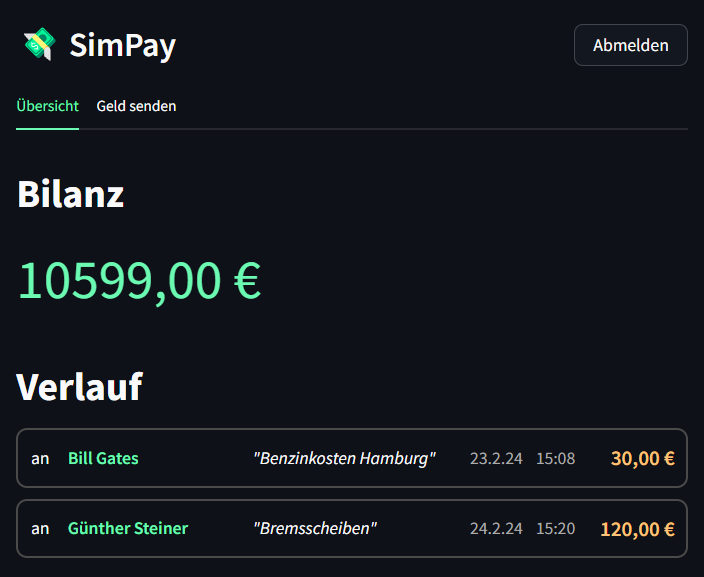
\includegraphics[width=.95\linewidth]{figures/impl/simpay_bilanz.png}
      \caption{Übersicht}
    %   \label{fig: blue totp app screenshot nicht verbunden}
    \end{subfigure}%
    \begin{subfigure}{.5\textwidth}
      \centering
      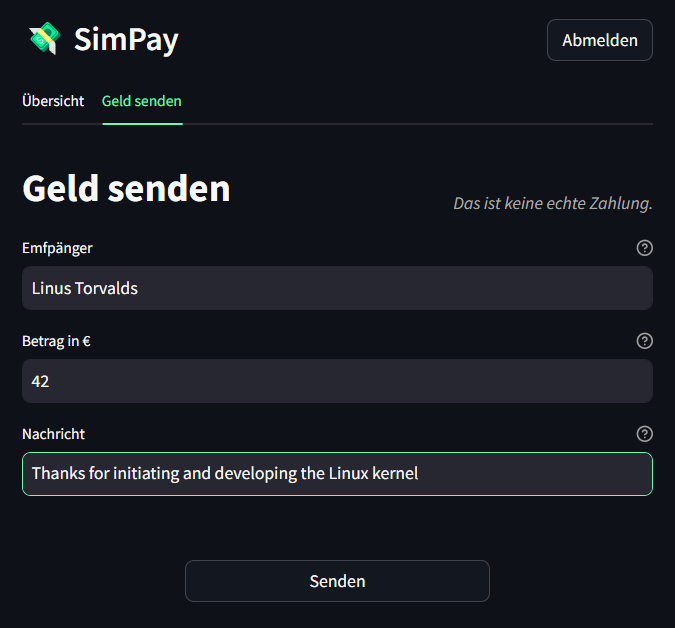
\includegraphics[width=.95\linewidth]{figures/impl/simpay_send.png}
      \caption{Überweisung}
    %   \label{fig: blue totp app screenshot verbunden}
    \end{subfigure}
    \caption[Website des fiktiven Dienstes Simpay]{Website des fiktiven Dienstes Simpay}
    \label{fig: simpay}
\end{figure}
\\\\
Der Webdienst wurde mit Streamlit\footnote{\href{https://streamlit.io/}{https://streamlit.io/}} (Python) als Frontend bzw. Host-Framework und 
einem eigens erstellten User Management und Logging entwickelt. Die Software wurde 
in einem Docker-Container auf einem Server des Instituts für Informatik der TU 
Bergakademie Freiberg gehostet. Die Verbindung zur Website wurde durch HTTPS 
gesichert. Die Passwörter der Teilnehmer werden mit der \textit{Password-Based Key 
Derivation Function 2} unter Verwendung des SHA256-Algorithmus, einer 
Iterationsanzahl von $700.000$ und einem 16 Byte langen Salt gehasht und 
gespeichert.